\documentclass{article}

\usepackage[english]{babel}
\usepackage[letterpaper,top=2cm,bottom=2cm,left=3cm,right=3cm,marginparwidth=1.75cm]{geometry}
\usepackage{amsmath}
\usepackage{graphicx}
\usepackage[colorlinks=true, allcolors=blue]{hyperref}
\usepackage{minted}
\usepackage{setspace}
\doublespacing
\title{Stock Prediction}
\author{Junwen Li, Zhixuan Zou}

\begin{document}
\maketitle


\section{Introduction}
Nowadays, quantitative investment technology based on mathematical models has been widely used and brought considerable returns to investors. Nowadays, artificial intelligence and machine learning technologies are on the ascendant, and they have made remarkable achievements in many fields such as image recognition and search recommendation. Compared with time series analysis, machine learning models can quickly process and analyze massive data and often have better generalization ability.

The stock is the most important part of the financial market, and it is a complex nonlinear dynamic system affected by many factors. It has become a subject of continuous research by scholars for a long time. The investment strategy is very important, so the stock forecasting model has important research significance. With the rapid development of computer technology and the arrival of the era of big data, neural network machine learning and deep learning technology have been greatly developed. Because of their strong nonlinear approximation ability and self-learning ability, they are widely used in time series forecasting, prompting stock research to enter a new stage. Among them, the recurrent neural network has outstanding performance in processing serialized data, has memory function, can save historical information, and can continuously update with the input of new data, which can effectively solve the long-term and short-term dependence of time series. Building machine learning is one approach to forecasting. Building machine learning models to predict stocks is indeed an interesting field. Both Python and Keras can build machine learning to predict stock trends, and today we are going to discuss how to use them to build a machine learning model to predict stock trends.

\section{Theory}

\subsection{Neural Networks}

We will be using The neural networks method in the data science model. Neural networks are also known as Artificial neural networks (ANN), and it is a core subset of machine learning. 
The neural network is a series of algorithms that mimic the way the brain recognizes relationships in a set of data. The neural network refers to a system of neurons, whether organic or artificial.

\subsection{Why Are Neural Networks Important}
In the absence of humanitarian assistance, neural networks can help computers make intelligent decisions because they can learn and model nonlinear and complex relationships between input and output data.

\subsection{What Can Neural Networks Do}
\begin{itemize}
    \item Medical diagnosis by medical image classification
    \item Targeted marketing by social network filtering and behavioral data analysis
    \item Financial predictions by processing historical data of financial instruments
    \item Electrical load and energy demand forecasting
    \item Process and quality control
    \item Chemical compound identification
\end{itemize}

\section{Implementation}
\subsection{Importing Libraries}
We will first import some of the most basic libraries or initial uses.
\begin{minted}{python}
import numpy as np
import pandas as pd
import talib
\end{minted}
Numpy is a fundamental package for computer science that we will use to perform computations on data sets. Import Numpy with the np alias.

Pandas can help us use the powerful data frame object, which will be used all the time in the process of building neural networks in Python.

Talib is a technical analysis library that can be used to calculate data such as RSI and Williams \%R indicators(William Percent Range) in the stock market.

\subsection{Setting Random Seed Numbers}
\begin{minted}{python}
import random
random.seed(42)
\end{minted}
We use the random.seed method to initialize the seed and give it a fixed number so that the initial number will be the same every time we run our code.

\subsection{Importing Data Set}
\begin{minted}{python}
dataset = pd.read_csv('RELIANCE.NS.csv')
dataset = dataset.dropna()
dataset = dataset[['Open', 'High', 'Low', 'Close']]
\end{minted}
Then we import the data set of RELIANCE on the New York Stock Exchange.

The data set is in CSV format, and the name is set to "RELIANCE.csv" (here we just take the company's stock data as an example, and you can choose the data to set yourself in practice). We use the Pandas library for this step, and the data is stored in a data frame called Dataset. We then drop missing values in the data set with the dropna() function. The data set contains the stock OHLC of Reliance Industries Group on the New York Stock Exchange from January 2000 to October 2017, i.e. daily open, high, low, and close prices. We only take OHLC data in the data set, which also includes trading hours, stock-adjusted prices, and stock trading volumes. We'll create our input features with OHLC values.

\subsection{Preparing Data Set}
\begin{minted}{python}
dataset['H-L'] = dataset['High'] - dataset['Low']
dataset['O-C'] = dataset['Close'] - dataset['Open']
dataset['3day MA'] = dataset['Close'].shift(1).rolling(window = 3).mean()
dataset['10day MA'] = dataset['Close'].shift(1).rolling(window = 10).mean()
dataset['30day MA'] = dataset['Close'].shift(1).rolling(window = 30).mean()
dataset['Std_dev']= dataset['Close'].rolling(5).std()
dataset['RSI'] = talib.RSI(dataset['Close'].values, timeperiod = 9)
dataset['Williams %R'] = talib.WILLR(dataset['High'].values
dataset['Low'].values, dataset['Close'].values, 7)
\end{minted}
Then we prepare the required input features, use them to train the neural network, and make predictions about stocks. We define the following input features:
\begin{itemize}
    \item The difference between the highest price and the lowest price
    \item The difference between the opening price and the closing price
    \item 3-day moving average
    \item 10-day moving average
    \item 30-day moving average
    \item Average variance over 5 days
    \item Relative strength index
    \item Williams \%R indicators
\end{itemize}
Moving Average: Referred to as MA, and refers to the use of statistical analysis methods to average stock prices (indexes) within a certain period of time, and connect the average values at different times to form an MA, which is used to observe stocks A technical indicator of the trend of stock price changes.

Relative Strength Index: Referrer to as RSI. It refers to analyzing the intention and strength of buying and selling orders in the market by comparing the average closing up and down in a period of time, so as to make future market trends.

Williams \%R: Abbreviated as W\%R. it is an oscillating indicator that measures whether a stock/index is overbought or oversold according to the swing point of the stock price. It measures the ratio of the distance between the peak (the highest price) created by both long and short sides to the daily closing price and the stock price fluctuation range within a certain period of time (such as 7 days), so as to provide a signal for the reversal of the stock market trend.

\begin{minted}{python}
dataset['Price_Rise'] = np.where(dataset['Close'].shift(-1) > dataset['Close'], 1, 0)
\end{minted}
Then we define the output value as the stock price increase, which is a binary variable that will be stored as 1 when the next day's closing price is higher than the current day's closing price.
\begin{minted}{python}
dataset = dataset.dropna()
\end{minted}
Then we use the dropna() function to drop all rows containing NaN values.
\begin{minted}{python}
X = dataset.iloc[:, 4:-1]
y = dataset.iloc[:, -1]
\end{minted}
Next, create two data frames "X" and "y" to store the input and output variables. The data frame "X" stores the input features, and its columns start at the 5th column (index 4) of the data set and go down to the 2nd last column. The last column will be stored in the data frame "y", which is the value we want to predict, which is the price increase.

\subsection{Spliting Data Set}
\begin{minted}{python}
split = int(len(dataset)*0.8)
X_train, X_test, y_train, y_test = X[:split], X[split:], y[:split], y[split:]
\end{minted}
In this segment of the code, we split the input and output variables to create a test data set and a training data set. Do this by creating a variable called split and defining it as an integer that is 0.8 times the length of the data set.

Then we split the variables of X and y into 4 separate data frames: X\_train, X\_test, y\_train, and y\_test. Any machine learning model will involve this step, the model will use the training data set to obtain the weights, and the test data set to see the performance of the model on new data. The test data set also contains the actual values of the output, which can help us understand the effect of the model. Later we will look at the confusion matrix in the code, which can be used to measure the prediction accuracy of the model.

\subsection{Feature Scaling}
\begin{minted}{python}
from sklearn.preprocessing import StandardScaler
sc = StandardScaler()
X_train = sc.fit_transform(X_train)
X_test = sc.transform(X_test)
\end{minted}
Normalizing the data set is another significant step in preprocessing data. 
This step will make the mean of all input features equal to 0 and convert their variance to 1. This ensures that the model is not biased by differences in input features when training the model. If this step is not handled well, the model may get confused and give higher weight to those input features with higher mean values.

We do this by importing the StandardScaler method from sklearn.preprocessing library. The variable sc is first instantiated with the StandardScaler() function, and then these changes are also applied to the X\_train and X\_test data sets with the fit\_transform function. Since the y\_train and y\_test data sets contain binary values, they do not need to be normalized.

Now that our data set is ready to be used, next we can build the neural network using the Keras library.

\subsection{Building Neutral Networks}
\begin{minted}{python}
from keras.models import Sequential
from keras.layers import Dense
from keras.layers import Dropout
\end{minted}
Now we import the functions used to build the neural network. Import the Sequential method from the Keras.models library, which is used to build the layers of the neural network sequentially. The next method we import is the Dense function from the Keras.layers library, which we will also use to build the layers of our neural network.
\begin{minted}{python}
classifier = Sequential()
\end{minted}
We instantiate the Sequential() function as a variable classifier. It will be used later when building the layers of the neural network in Python.
\begin{minted}{python}
classifier.add(Dense(units = 128, kernel_initializer = 'uniform', activation = 'relu',
input_dim = X.shape[1]))
\end{minted}
We use the add() function to add layers to the classifier. The argument of the add() function is the Dense() function, which has the following arguments:
\begin{itemize}
    \item Units: It defines the number of nodes or neurons in a certain layer. We set the value here to 128, which means we will have 128 neurons in our hidden layer.
    \item Kernel\_initializer: It defines the starting values of the different neuron weights in the hidden layer. We define it as "uniform" here, meaning that all weights will be initialized with uniformly distributed values.
    \item Activation: It is the activation function of neurons in the hidden layer, here we define the activation function as a modified linear unit function.
    \item Input\_dim: It defines the number of inputs to be fed into the hidden layer, and we define the number of inputs to be equal to the number of columns in the input feature data frame. However, this argument is no longer needed in later layers, since the model knows how much output was generated in the previous layer.
\end{itemize}
\begin{minted}{python}
classifier.add(Dense(units = 128, kernel_initializer = 'uniform', activation = 'relu'))
\end{minted}
Then we add another layer, 128 neurons, with a kernel\_initializer with consistent weights, and the activation function is a rectified linear unit. In this neural network, we only build two hidden layers.
\begin{minted}{python}
classifier.add(Dense(units = 1, kernel_initializer = 'uniform', activation = 'sigmoid'))
\end{minted}
Then we build the output layer, only one output is needed, so Units are set to 1, and the sigmoid function is selected as the activation function because we want to predict the probability of stock market changes.
\begin{minted}{python}
classifier.compile(optimizer = 'adam', loss = 'mean_squared_error', 
metrics = ['accuracy'])
\end{minted}
Finally, pass in the following arguments to compile the classifier:
\begin{itemize}
    \item Optimizer: Select the optimizer as "Adam", which is an extended form of the stochastic gradient descent algorithm.
    \item Loss: It defines the loss that needs to be optimized during the training process. We define loss as the mean square error.
    \item Metrics: It defines the matrix that the model evaluates during training and testing. We choose accuracy as the evaluation matrix for the model.
\end{itemize}
\begin{minted}{python}
classifier.fit(X_train, y_train, batch_size = 10, epochs = 100)
\end{minted}
Now we need to fit the created neural network to the training data set by passing X\_train, y\_train, batch size, and the number of epochs to the fit() function. The batch size refers to the data points that the model uses to calculate the error before backpropagating the error and modifying the weights. The number of epochs refers to the number of times to train the model with the training set.

In this way, the model is built, and after the model is trained and evaluated, the model can be used to predict the stock market.

\subsection{Predicting the Movement of the Stock}
\begin{minted}{python}
y_pred = classifier.predict(X_test)
y_pred = (y_pred > 0.5)
\end{minted}
We make predictions using the predict() function. Passing X\_test into the model as an argument, and saving the result as a variable named y\_pred. Then we convert y\_pred under the condition of y\_pred > 5 to save the binary value. Now the variable y\_pred holds True or False depending on whether the predicted value is greater than 0.5.
\begin{minted}{python}
dataset['y_pred'] = np.NaN
dataset.iloc[(len(dataset) - len(y_pred)):,-1:] = y_pred
trade_dataset = dataset.dropna()
\end{minted}
Next, we create a new column in the data frame titled "y\_pred" and store the NaN values in the column. We then save the y\_pred values into this new column, starting with the rows of the test set. This can be done by splitting the data set using the iloc method (code above). Then we drop all NaN values from the data set and save them as a new data frame named trade\_dataset.

\subsection{Calculation of Model Returns}
\begin{minted}{python}
trade_dataset['Tomorrows Returns'] = 0.
trade_dataset['Tomorrows Returns'] = np.log(trade_dataset['Close']/
trade_dataset['Close'].shift(1))
trade_dataset['Tomorrows Returns'] = trade_dataset['Tomorrows Returns'].shift(-1)
\end{minted}
Now that we have the predicted value of the stock price movement, we can calculate the return of the model making the prediction. If the value of y is True, we will take a long trade, if it is False, we will take a short trade.

We first calculate the market return at the close of the next day if we take a long trade at the close of the day. First, we create a new column in trade\_dataset named "Tomorrows Returns" and save it as value 0. We represent the floating point values stored in the new column in decimal notation. Next, we save this as the day's log return, which is the logarithm of yesterday's closing price divided by today's closing price. We then move these values up by one element so that the next day's earnings are saved at that day's share price.
\begin{minted}{python}
trade_dataset['Strategy Returns'] = 0.
trade_dataset['Strategy Returns'] = np.where(trade_dataset['y_pred'] == True,
trade_dataset['Tomorrows Returns'], - trade_dataset['Tomorrows Returns'])
\end{minted}
Next, we calculate the model return, create a new column titled "Strategy\_Returns" and initialize it with 0. (indicating storing a floating point value). Using the np.where() function, then if the "y\_pred" column is True (long trade), we will save the value in the column "Tomorrow Returns", otherwise we will save the value in the column "Tomorrow Returns" (short trade) Negative values are saved into the column "Strategy\_Returns".
\begin{minted}{python}
trade_dataset['Cumulative Market Returns']=np.cumsum(trade_dataset['Tomorrows Returns'])
trade_dataset['Cumulative Strategy Returns'] = 
np.cumsum(trade_dataset['Strategy Returns'])
\end{minted}
Now we calculate the cumulative return of the market and the model. These values are calculated using the cumsum() function. We'll use the cumulative sum to plot the market return and the model return from the previous step.

\subsection{Drawing a Profit Graph}
\begin{minted}{python}
import matplotlib.pyplot as plt
plt.figure(figsize=(10,5))
plt.plot(trade_dataset['Cumulative Market Returns'], color='r', label='Market Returns')
plt.plot(trade_dataset['Cumulative Strategy Returns'], color='g', 
label='Strategy Returns')
plt.legend()
plt.show()
\end{minted}
Now we draw a visualization of market returns and our model returns, visually showing the comparison between the model effect and the market effect.

We import matplotlib.pyplot, and then use the plot function to plot the market return versus the model return based on the cumulative values stored in the data frame trade\_dataset. We then create and display the legend using the legend() and show() functions, respectively. The figure below is the output of the code. The green line represents the model return and the red line represents the market return.
\begin{figure}[h!]
\centering
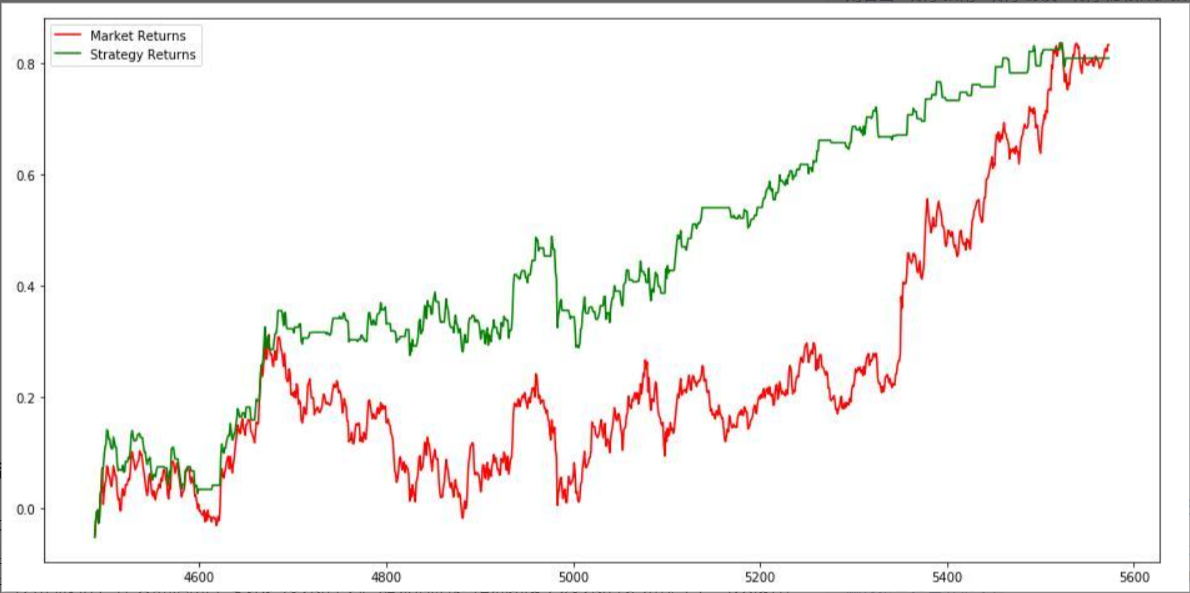
\includegraphics[width=0.3\textwidth]{result.png}
\caption{\label{fig:result}The result of the stock prediction}
\end{figure}


\subsection{Conclusion}
In this practice, we learned how to build a neural network from scratch using Python, Keras, etc. for stock trading. If there is enough data and enough training times, the performance of the neural network can be further improved. The model built in this article is relatively simple and mainly based on daily stock prices. In reality, it is much more complicated than this. If you want to build and train a more complex trading model, you can use the stock market data detailed every minute, so that you can get enough data and the training effect of the model is more efficient.

\section{Data}
We collect the data from \url{https://github.com/mehul90/NSE_TRADER/blob/master/data/RELIANCE2000-01-012017-10-29.csv}

\section{Reference}
\url{https://www.investopedia.com/terms/n/neuralnetwork.asp}

\url{https://aws.amazon.com/what-is/neural-network/#:~:text=with%20greater%20accuracy.-,Why%20are%20neural%20networks%20important%3F,that%20are%20nonlinear%20and%20complex.}

\url{https://github.com/mehul90/NSE_TRADER/blob/master/data/RELIANCE2000-01-012017-10-29.csv}
\end{document}



